\documentclass[11pt,letterpaper]{article}
\usepackage[utf8]{inputenc}
\usepackage[left=1in,right=1in,top=1in,bottom=1in]{geometry}
\usepackage{amsfonts,amsmath}
\usepackage{graphicx,float}
\usepackage{esint}
\usepackage{csquotes}
% -----------------------------------
\usepackage{hyperref}
\hypersetup{%
  colorlinks=true,
  linkcolor=blue,
  citecolor=blue,
  urlcolor=blue,
  linkbordercolor={0 0 1}
}
% -----------------------------------
\usepackage[authordate,backend=biber]{biblatex-chicago}
\addbibresource{citation.bib}
% -----------------------------------
\usepackage{fancyhdr}
\newcommand\course{MATH-UA.0230, PHYS-UA 180\\Introduction to Fluid Dynamics}
\newcommand\hwnumber{3}                  % <-- homework number
\newcommand\NetIDa{Ryan Sh\`iji\'e D\`u} 
\newcommand\NetIDb{February 16th, 2023}
\pagestyle{fancyplain}
\headheight 35pt
\lhead{\NetIDa\\\NetIDb}
\chead{\textbf{\Large Worksheet \hwnumber}}
\rhead{\course}
\lfoot{}
\cfoot{}
\rfoot{\small\thepage}
\headsep 1.5em
% -----------------------------------
\usepackage{titlesec}
\renewcommand\thesubsection{(\arabic{section}.\alph{subsection})}
\titleformat{\subsection}[runin]
        {\normalfont\bfseries}
        {\thesubsection}% the label and number
        {0.5em}% space between label/number and subsection title
        {}% formatting commands applied just to subsection title
        []% punctuation or other commands following subsection title
% -----------------------------------
\setlength{\parindent}{0.0in}
\setlength{\parskip}{0.1in}
% -----------------------------------
\newcommand{\de}{\mathrm{d}}
\newcommand{\DD}{\mathrm{D}}
\newcommand{\pe}{\partial}
\newcommand{\mcal}{\mathcal}
%\newcommand{\pdx}{\left|\frac{\partial}{\partial_x}\right|}

\newcommand{\dsp}{\displaystyle}

\newcommand{\norm}[1]{\left\Vert #1 \right\Vert}
%\newcommand{\mean}[1]{\left\langle #1 \right\rangle}
\newcommand{\mean}[1]{\overline{#1}}
\newcommand{\inner}[2]{\left\langle #1,#2\right\rangle}

\newcommand{\ve}[1]{\boldsymbol{#1}}

\newcommand{\thus}{\Rightarrow \quad }
\newcommand{\fff}{\iff\quad}
\newcommand{\qdt}[1]{\quad \mbox{#1} \quad}

\renewcommand{\Re}{\mathrm{Re}}
\renewcommand{\Im}{\mathrm{Im}}
\newcommand{\E}{\mathbb{E}}
\newcommand{\lap} {\nabla^2}
\renewcommand{\div}{\nabla\cdot}

\newcommand{\csch}{\text{csch}}
\newcommand{\sech}{\text{sech}}


\newcommand{\hot}{\text{h.o.t.}}

\newcommand{\ssp}{\left.\qquad\right.}

\newcommand{\var}{\text{var}}
\newcommand{\cov}{\text{cov}}


\begin{document}

\section{Derivation of the Lamb vector}
A useful vector identity in fluid mechanics is
\begin{align}
    \ve v(\nabla\cdot\ve v) = \frac{1}{2}\nabla\ve v^2-\ve v\times\ve \omega.\label{eq:lamb_ident}
\end{align}
For example, we use this identity in the derivation of the Bernoulli's principle. The Lamb vector is defined as
\begin{align}
    \ve\ell = \ve v\times\ve \omega.
\end{align}
We will derive the the vector identity \eqref{eq:lamb_ident}.

\subsection{}
Show that the cross product can be written as
\begin{align}
    \ve a\times \ve b = \epsilon_{ijk}a_ib_j\ve e_{(k)}
\end{align}
where $\epsilon_{ijk}$ is the permutation symbol:
\begin{align}
    \epsilon_{ijk} = \begin{cases}
        0 &\text{, if any two of $i,j,k$ are the same}\\
        1 &\text{, if $i,j,k$ is an even permutation of $1,2,3$}\\
        -1 &\text{, if $i,j,k$ is an odd permutation of $1,2,3$}.
    \end{cases}
\end{align}

\subsection{}
[From \cite{Aris_62}, Exercise 2.32.1] Show by enumerating typical cases that
\begin{align}
    \epsilon_{ijk}\epsilon_{k\ell m} = \delta_{i\ell}\delta_{jm}-\delta_{im}\delta_{j\ell}.\label{eq:perm_prod_ident}
\end{align}

\subsection{}
Use \eqref{eq:perm_prod_ident} to show \eqref{eq:lamb_ident}.

\newpage
\section{Bernoulli's principle: examples}
\subsection{Flow out of a water tank}
Imagine a water tank with height $h$ of water inside. At the bottom there is a small hole. What would be the speed of the water flowing out of the hole.

\subsection{Venturi effect}
Calculate the fluid velocity difference at position 1 and 2
\begin{figure}[H]
    \centering
    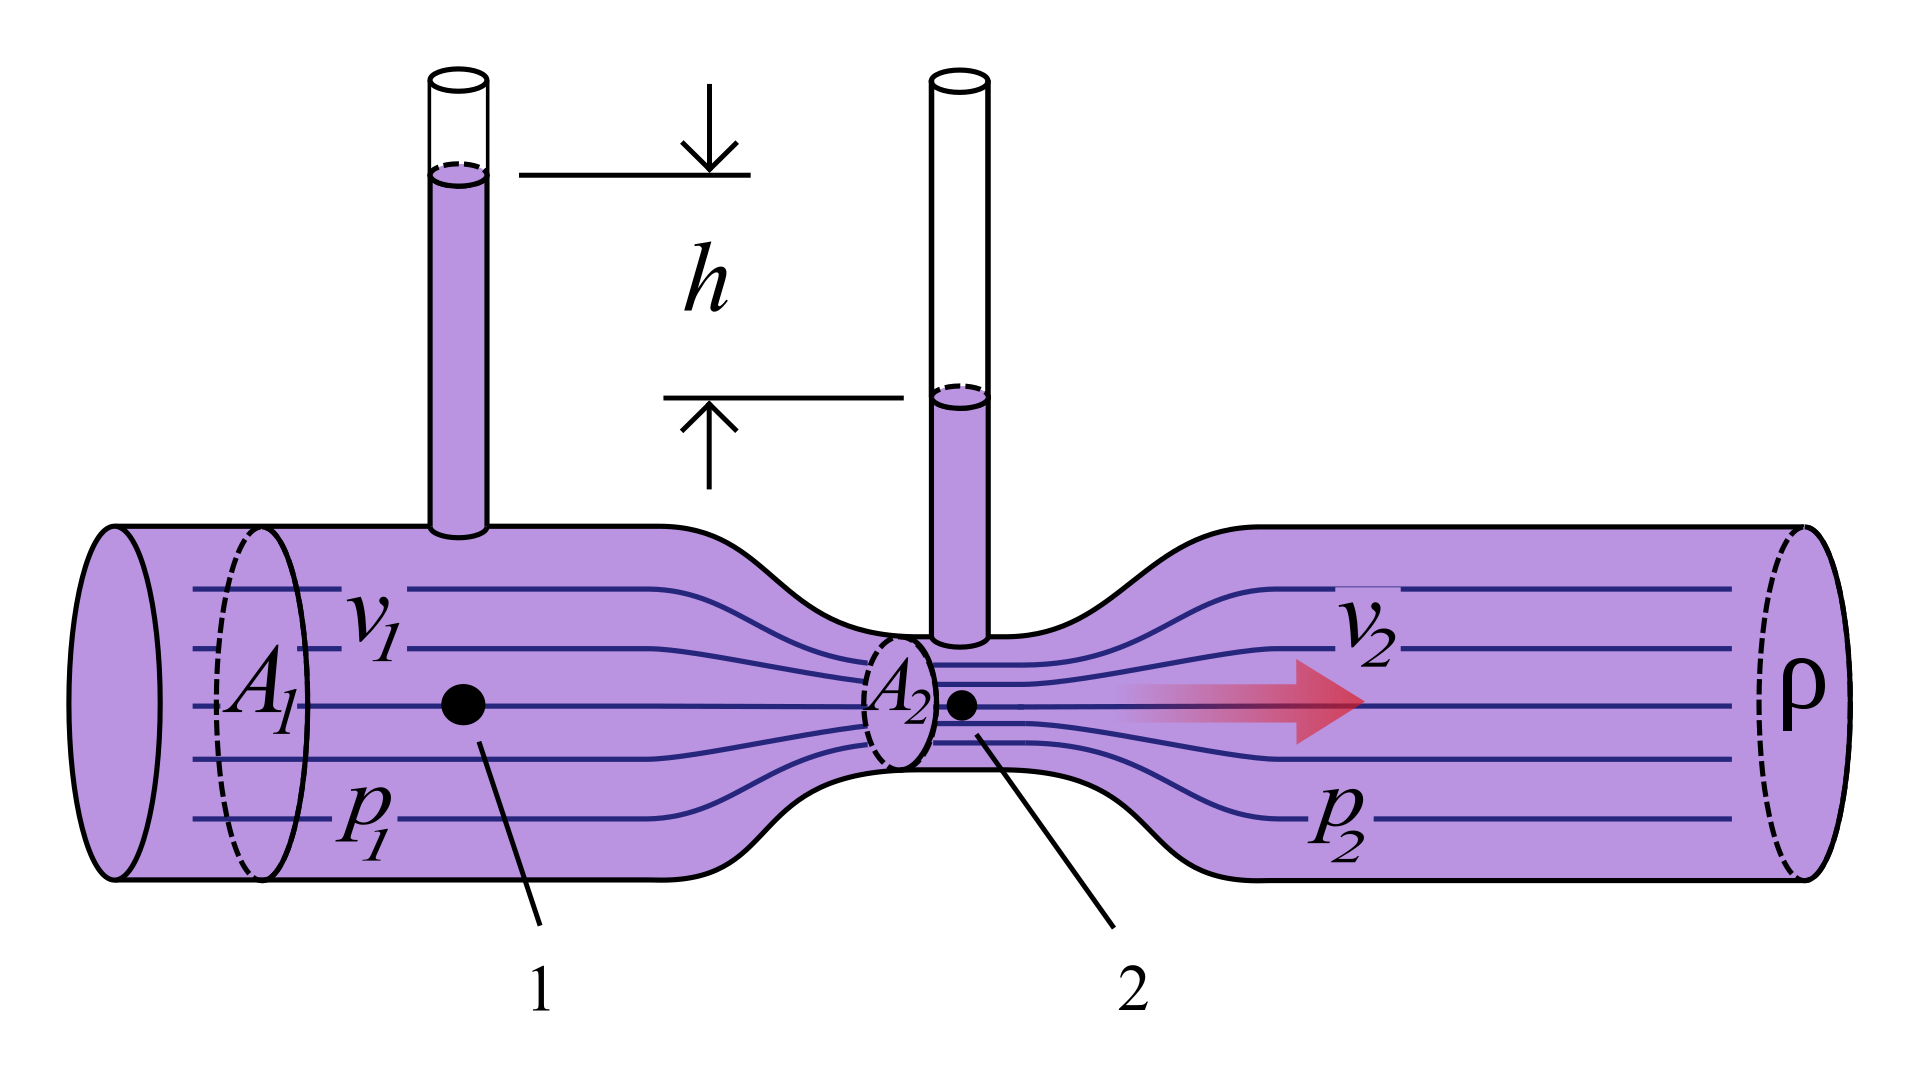
\includegraphics[width=0.5\textwidth]{figs/Venturi_wiki}
\end{figure}

\subsection{Pitot's tube}
Using the idea of the above device, think of a device that measures the speed of the fluid flow.

\newpage
\section{The ABC flows}
By using \eqref{eq:lamb_ident}, we can write the incompressible Euler equation as
\begin{align}
    &\frac{\pe\ve v}{\pe t}+\ve\omega\times\ve v = -\nabla H,\\
    &\nabla\cdot\ve v = 0.
\end{align}
where $H$ is the energy
\begin{align}
    H = \frac{p}{\rho}+\frac{1}{2}\ve v^2.
\end{align}
The Arnold, Beltrami, Childress (ABC) flow is an interesting steady state solution of Euler. It has the velocity field on the $2\pi$-periodic 3D domain
\begin{align}
    \begin{cases}
        u= A\sin z+C\cos y\\
        v= B\sin x+A\cos z\\
        w= C\sin y+B\cos x\\
    \end{cases}
\end{align}
where $A,B$, and $C$ are constant parameters. Despite its simple appearance in the Eulerian frame, the Lagrangian behavior of this flow is presumably chaotic. To quote \cite{DombreEtAl_86} which named this flow
\begin{displayquote}
Three-dimensional steady flows with a simple Eulerian representation can have a chaotic Lagrangian structure. By this we mean that infinitesimally close fluid particles following the streamlines may separate exponentially in time, while remaining in a bounded domain, and that individual streamlines may appear to fill entire regions of space.
\end{displayquote}
and
\begin{displayquote}
    From a fluid dynamical viewpoint flows with chaotic streamlines are interesting because they may considerably enhance transport without being turbulent in the usual sense - they only display what might be called `Lagrangian turbulence'.
\end{displayquote}

We will be less ambitious and show some basic properties of this flow.
\subsection{}
Show the ABC flows are incompressible.

\subsection{}
Show the ABC flows are Beltrami flows. That is
\begin{align}
    \ve \omega\times\ve v = 0.
\end{align}
Hint: Show $\ve \omega = \ve v$. Why does this identity shows $\ve v$ is Beltrami?

\subsection{}
Conclude the ABC flows are exact solution to the steady state incompressible Euler equation.

    
\vfill
\printbibliography


\end{document}